% !TeX program = pdflatex
\documentclass[tikz,border=8pt]{standalone}
\usepackage{pgfplots}
\pgfplotsset{compat=1.16}
\definecolor{FigureBlue}{HTML}{2563EB}
\definecolor{FigureOrange}{HTML}{EA580C}
\definecolor{FigureSlate}{HTML}{475569}
\begin{document}
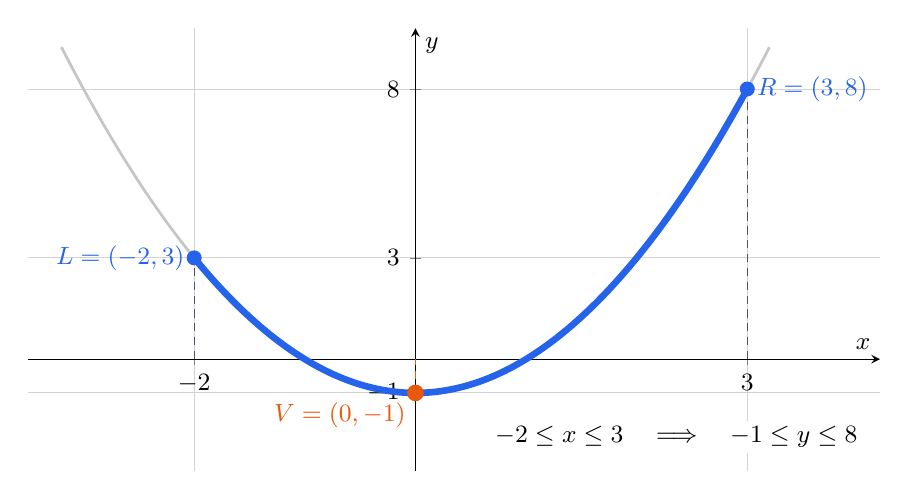
\begin{tikzpicture}
  \begin{axis}[
    width=12.4cm,
    height=7.2cm,
    axis lines=middle,
    xmin=-3.5, xmax=4.2,
    ymin=-3.3, ymax=9.8,
    xlabel={$x$}, ylabel={$y$},
    xtick={-2,0,3},
    ytick={-1,3,8},
    grid=both,
    minor tick num=1,
    grid style={line width=.2pt,draw=gray!20},
    major grid style={line width=.35pt,draw=gray!35},
    tick label style={font=\small},
    label style={font=\small},
    clip=false,
  ]
    \addplot[gray!45, line width=1pt, domain=-3.2:3.2, samples=161] {x^2-1};
    \addplot[FigureBlue, line width=2.4pt, domain=-2:3, samples=161] {x^2-1};
    \addplot[only marks, mark=*, mark size=2.5pt, FigureBlue]
      coordinates {(-2,3) (3,8)};
    \addplot[only marks, mark=*, mark size=2.8pt, FigureOrange]
      coordinates {(0,-1)};
    \draw[densely dashed, FigureSlate] (axis cs:-2,0) -- (axis cs:-2,3);
    \draw[densely dashed, FigureSlate] (axis cs:3,0) -- (axis cs:3,8);
    \draw[densely dashed, FigureOrange] (axis cs:0,-1) -- (axis cs:0,0);
    \node[anchor=east, text=FigureBlue, font=\small] at (axis cs:-2,3) {$L=(-2,3)$};
    \node[anchor=west, text=FigureBlue, font=\small] at (axis cs:3,8) {$R=(3,8)$};
    \node[anchor=north east, text=FigureOrange, font=\small] at (axis cs:0,-1) {$V=(0,-1)$};
    \node[anchor=south east, fill=white, inner sep=2pt, font=\small]
      at (axis cs:4.05,-2.8) {$-2\le x\le3\quad\Longrightarrow\quad-1\le y\le8$};
  \end{axis}
\end{tikzpicture}
\end{document}
